\begin{figure}[!h]
  \centering
  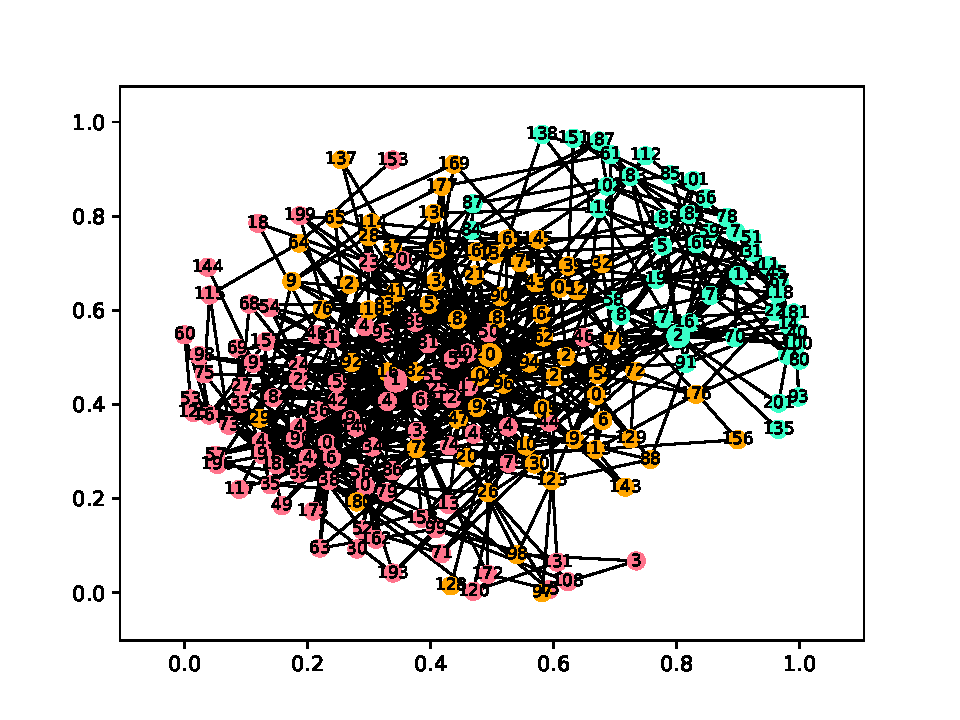
\includegraphics[trim={2.1cm 2cm 2cm 2cm}, clip, width=\columnwidth]{img/pdf/cover}
  \caption{News Spreading Network Simulation\protect\footnotemark}
  \label{fig:abstract}
\end{figure}
\footnotetext{Simulation run with: sources: 3, users: 200, cycles:800, average degree: 5, seed: 123456789}
\section*{Abstract}\label{abstract}
Our aim is to analyse the influence of memory in a news spreading dynamic.
In order to do that, we have built a framework of agents connected in a
network and equipped them with a set of basic functions. We wish to
observe a diffusion-like process.\\
In this paper we expose the underlying
methodology and try to explain it with a simple tutorial.

\section{Introduction}\label{sec:introduction}
For the purpose of modeling the interactions between users in the
context of news spreading, it is convenient to talk about autonomous agents
linked by friendly ties whose overall view constitutes the network.
Network population is made of two breeds of agents: sources and users.
These two breeds will interact in an autonomous approach during
program execution.
The network is initially a random connection of agents and modifies
its own topology following a set of microscopic agents' actions.\\
We believe that news' content and agents social impact give rise to natural
news diffusion in a social-like network.
We hope to observe a spontaneous growth of scale-free regime starting
from dynamical micro-interactions.\\
We also hope to reveal a natural segregation behaviour that subjugate
a great deal of real social networks. In addition to these items
we wonder if there can be correlation between news spreading and agents'
memory lenght. In practice, we have worked with
the Swarm-like protocol in python 3 named SLAPP3.\footnote{For
  reference and download from: \url{https://github.com/terna/SLAPP}}

\section{Overview}\label{sec:overview}
We have built our model focusing on two methodologies:
agent based and network frameworks. We have blended these two
frames considering a network of agents. 
\subsection{Context}
Let us focus on the dynamical process of news spreading in a social\footnote{The word \textit{social} can be thought in a general context.} network.\\
News diffusion is generally studied in a stochastic context, ruled by a
set of stochastic differential equations.\cite{chen2013information}
There is an apparent similarity with epidemiological processes. 
However, while epidemic diffusion becomes a viral process, when a
threshold is exceeded, news spreading process seems to be threshold-less.
The epidemic model of information diffusion is usually a compartmental model
in which agents coexist in the world in different
stages.\cite{barrat2008dynamical}
Most of initial users stay in the compartment of \textit{ignorants} whereas
a minority of them stay in the \textit{spreader} compartment.
There is another compartment, the \textit{stiflers}: users influenced by news
who do not spread anymore (equivalent to \textit{recovery} in the
SIR\footnotemark model).\footnotetext{Acronym of Susceptible-Infected-Recovery, most famous model of epidemic spreading.}\\
This \textit{Spreader-Ignorant-stifler} model (SIs) can be sketched by a set
of transitions between compartments; one of the transition is spontaneous
while the others are induced by contact:
%
\begin{itemize}
\item$ I \longrightarrow S$
\item $S+I \longrightarrow S + S$

\item $S + S \longrightarrow s + S$

\item $s + S \longrightarrow  s + s$
\end{itemize}
%
$S$ is the \textit{Spreader}, $I$ is the \textit{Ignorant} and $s$
the \textit{stifler}. 
The first process corresponds to the spontaneous transition from the ignorant
to spreader compartment; the second one corresponds to
the contamination of an ignorant by contact with a spreader; 
the third and fourth interactions reproduce transitions by contact
to the stifler compartment. Dynamic evolution is governed by
series of transitions from a compartment to another one.
Just as all spreaders reach the stifler compartment, ignorants
remain so and the epidemic stops.\\
This approach is applicable to a network of users to predict the reproductive 
number\footnote{The reproductive number $R_{0}$ is defined by characteristic
  parameters that affect spreading like average degree (in first
  approximation) and diffusion rate. } 
which enable us to estimate the future qualitative behaviour of spreading: 
if this number is above some epidemic threshold then virality of diffusion
is guaranteed.\\
This can be a reliable description for a single news viral diffusion, but
when we deal with multiple news, the analysis by a set of several
differential equations would result more difficult.\\
A compartmental approach to study the phenomenon of information diffusion
has been widely examined in the last years, with very different variants
of naive models.\cite{fedewa2013spread}\cite{tambuscio2016network}
There are also several papers underlining interesting results in social
science: for example social influence, infection,
segregation,\cite{henry2011emergence} homophily\cite{aiello2012friendship}
or fake news diffusion;\cite{tambuscio2016network}\cite{nekovee2007theory}
the effects of fact-checking or bot-agent insertion\cite{aiello2012people}
in a network are studied too.
In news spreading literature, only few models are built on an agent
architecture.\cite{liu2011rumor}\cite{serrano2015novel}\cite{seo2012identifying}\cite{de2013simulation}\cite{serrano2016validating}

\subsection{Why Agents?}\label{subsec:whyagents}
Agents are a very useful paradigm to model social
interactions.\cite{axtell2000agents}
They can operate in their environment, take decisions and interact with
each other.
There is no communication protocol between them but they communicate
and share news with "friends".\\
The environment is not deterministic. 
Every action can produce different effects with a different probability,
but the simulation must be reproducible.
Actions between agents are non-deterministic: they don't have complete
control of another agent and have limited senses and sensors.\\
The required characteristics of each agent
are:\cite{wooldridge1995intelligent}
%
\begin{itemize}
\item [\textit {rationality:}] agents can take choices depending on their
  own belief and their surrounding environment;
\item [\textit {reactivity:}] agents can check the world clock and news
  spreading nearby during the dynamic;
\item [\textit {proactiveness:}] agents can express their own will,
  taking autonomous initiatives;
\item [\textit {social ability:}] they know how to send and receive news,
  to determine sympathy with neighbours;
\item [no \textit{mobility}] is required. 
\end{itemize}
%
Each agent can receive information from the world or from another agent;
it\footnote{There is no sexual division among agents} can also interact
with the world or with an agent, in order to meet its own ``character''
(a.k.a. state of mind).
They can modify their surrounding environment by means of the adding
and removal of edges in social network.
The only accessible variable for each agent is the clock number; they
can also access some neighbours' information.\\
Each agent makes local fair decisions: global behaviours may emerge.
When active, each agent can control the environment and reacts to the changes. 
During the inactive state the environment can change so an agent's previous
buffered actions may not be performed.
For this reason the agent can act unpredictably and somehow irrational.
